\documentclass[tikz,margin=2mm]{standalone}
\usetikzlibrary{positioning}
\usetikzlibrary{shapes.geometric}

\begin{document}

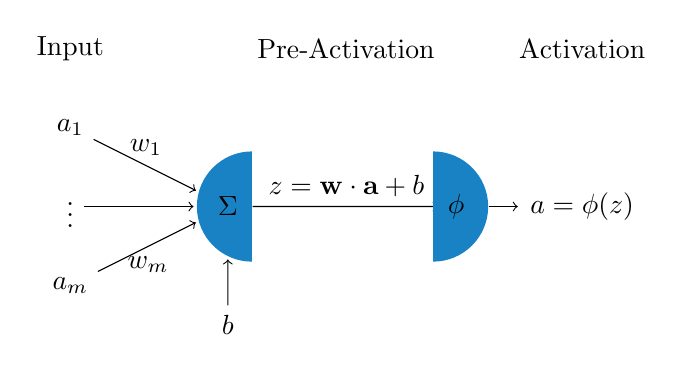
\begin{tikzpicture}[shorten >=1pt,->]
    \definecolor{hid}{HTML}{1982c4}
    \node[name=sc1,shape=semicircle, fill=hid, shape border rotate=90, minimum width=1.4cm] at (2, -2) {$\Sigma$};{};
    \node (x-1) at (0,-1) {$a_1$};
    \node (x-dots) at (0,-2) {\vdots};
    \node (x-m) at (0,-3) {$a_m$};

    \path (x-1) edge node[midway, above] {$w_1$} (sc1);
    \path (x-dots) edge (sc1);
    \path (x-m) edge node[midway, below] {$w_m$} (sc1);

    \node[below of=sc1, node distance=1.5cm] (b) {$b$};
    \path (b) edge (sc1);

    \path (sc1) edge node[above] {$z=\mathbf{w}\cdot\mathbf{a}+b$} (4.7, -2);
    \node (preact) at (3.5,-0) {Pre-Activation};

    \node[name=sc2,shape=semicircle, fill=hid, shape border rotate=270, minimum width=1.4cm] at (4.9, -2) {$\phi$};{};
    \node (a) at (6.5, -2) {$a=\phi(z)$};
    \path (sc2) edge (a);
    \node (act) at (6.5,-0) {Activation};
    \node (inp) at (0,0) {Input};
\end{tikzpicture}

\end{document}
